%!TEX encoding = UTF-8 Unicode

\begin{figure*}
  \tikzstyle{affnode} = [ellipse, draw, thick]%fill=gray!20, thick]%node distance=1cm, text width=6em, text centered, minimum height=4em, thick]
  \tikzstyle{wordnode} = [ellipse, draw, thick]
  \tikzstyle{group} = [rectangle, draw, black, thick]%, inner sep=0.5cm
  \tikzstyle{dashedgroup} = [rectangle, draw, inner sep=0.6cm, dashed, rounded corners, black]
  \tikzstyle{dottedgrouptrapezium} = [trapezium, draw, dotted, rounded corners, black]
  \begin{minipage}{0.5\textwidth}
    \centering
    \begin{tikzpicture}
      % single nodes
      \node[affnode] (g1) {$g_1$};
      \node[affnode, right of=g1] (g2) {$g_2$};
      \node[right of=g2] (gdots) {$\dots$};
      \node[affnode, right of=gdots] (f1) [right=0.5cm] {$f_1$};
      \node[affnode, right of=f1] (f2) {$f_2$};
      \node[right of=f2] (fdots) {$\dots$};
      \node[affnode, below of=f1] (e2) [below=0.7cm] {$e_2$};
      \node[affnode, left of=e2] (e1) {$e_1$};
      \node[right of=e2] (edots) {$\dots$};
      \node[wordnode, below of=e1] (w1)  [below=0.7cm] {$w_1$};
      \node[wordnode, right of=w1] (w2) {$w_2$};
      \node[right of=w2] (wdots) {$\dots$};
      % groups
      \node[group, fit=(g1) (g2) (gdots),label=above:Gesture Features] (gestures) {};
      \node[group, fit=(f1) (f2) (fdots),label=above:Object Features] (features) {};
      \node[group, fit=(e1) (e2) (edots),label=above:Effects] (effects) {};
      \node[group, fit=(w1) (w2) (wdots),label=above:Words] (words) {};
      % arrows
      \draw[myarrow] (gestures) -- ([xshift=-30pt]effects.north);
      \draw[myarrow] (gestures) to [out=260,in=150] (words.west);
      \draw[myarrow] (features) -- ([xshift=20pt]effects.north);
      \draw[myarrow] ([xshift=20pt]features.south) to [out=280,in=30] (words.east);
      \draw[myarrow] ([xshift=30pt]effects.south) -- ([xshift=30pt]words.north);
      % extra
      \node[affnode, above of=gestures] (actions) [above=1cm] {Actions};
      \draw[myarrow] (actions) -- (gestures);
      \node[dashedgroup, fit=(gestures) (features) (effects) (words),label={[shift={(0:2.2)}]above:Observable variables}] (observable) {};
    \end{tikzpicture}

    \vspace{6mm}
    (a) ideal case
  \end{minipage}
  \begin{minipage}{0.5\textwidth}
    \centering
    \begin{tikzpicture}
      % single nodes
      \node[affnode] (g1) {$g_1$};
      \node[affnode, right of=g1] (g2) {$g_2$};
      \node[right of=g2] (gdots) {$\dots$};
      \node[group, fit=(g1) (g2) (gdots),label=above:Gesture Features] (gestures) {};
      \node[affnode, below of=gestures] (actions) [below=1cm] {Actions};
      \node[affnode, right of=actions] (f1) [right=1.6cm] {$f_1$};
      \node[affnode, right of=f1] (f2) {$f_2$};
      \node[right of=f2] (fdots) {$\dots$};
      \node[affnode, below of=f1] (e2) [below=0.7cm] {$e_2$};
      \node[affnode, left of=e2] (e1) {$e_1$};
      \node[right of=e2] (edots) {$\dots$};
      \node[wordnode, below of=e1] (w1)  [below=0.7cm] {$w_1$};
      \node[wordnode, right of=w1] (w2) {$w_2$};
      \node[right of=w2] (wdots) {$\dots$};
      % groups
      \node[group, fit=(f1) (f2) (fdots),label=above:Object Features] (features) {};
      \node[group, fit=(e1) (e2) (edots),label=above:Effects] (effects) {};
      \node[group, fit=(w1) (w2) (wdots),label=above:Words] (words) {};
      \node[dashedgroup, fit=(actions) (features) (effects) (words),label={[shift={(0:2.2)}]above:Affordance-word model}]{};
      % arrows
      \draw[myarrow] (actions) -- ([xshift=-30pt]effects.north);
      \draw[myarrow] (actions) to [out=260,in=150] (words.west);
      \draw[myarrow] (features) -- ([xshift=20pt]effects.north);
      \draw[myarrow] ([xshift=20pt]features.south) to [out=280,in=30] (words.east);
      \draw[myarrow] ([xshift=30pt]effects.south) -- ([xshift=30pt]words.north);
      % extra
      %\node[affnode, above of=actions] (gestures) [above=1cm] {Gesture Features};
      \draw[myarrow] (actions) -- (gestures);
      \node[dashedgroup, fit=(actions) (gestures),label=above:Gesture/Action recognition]{};
    \end{tikzpicture}

    (b) our model
  \end{minipage}
    %\centering
    %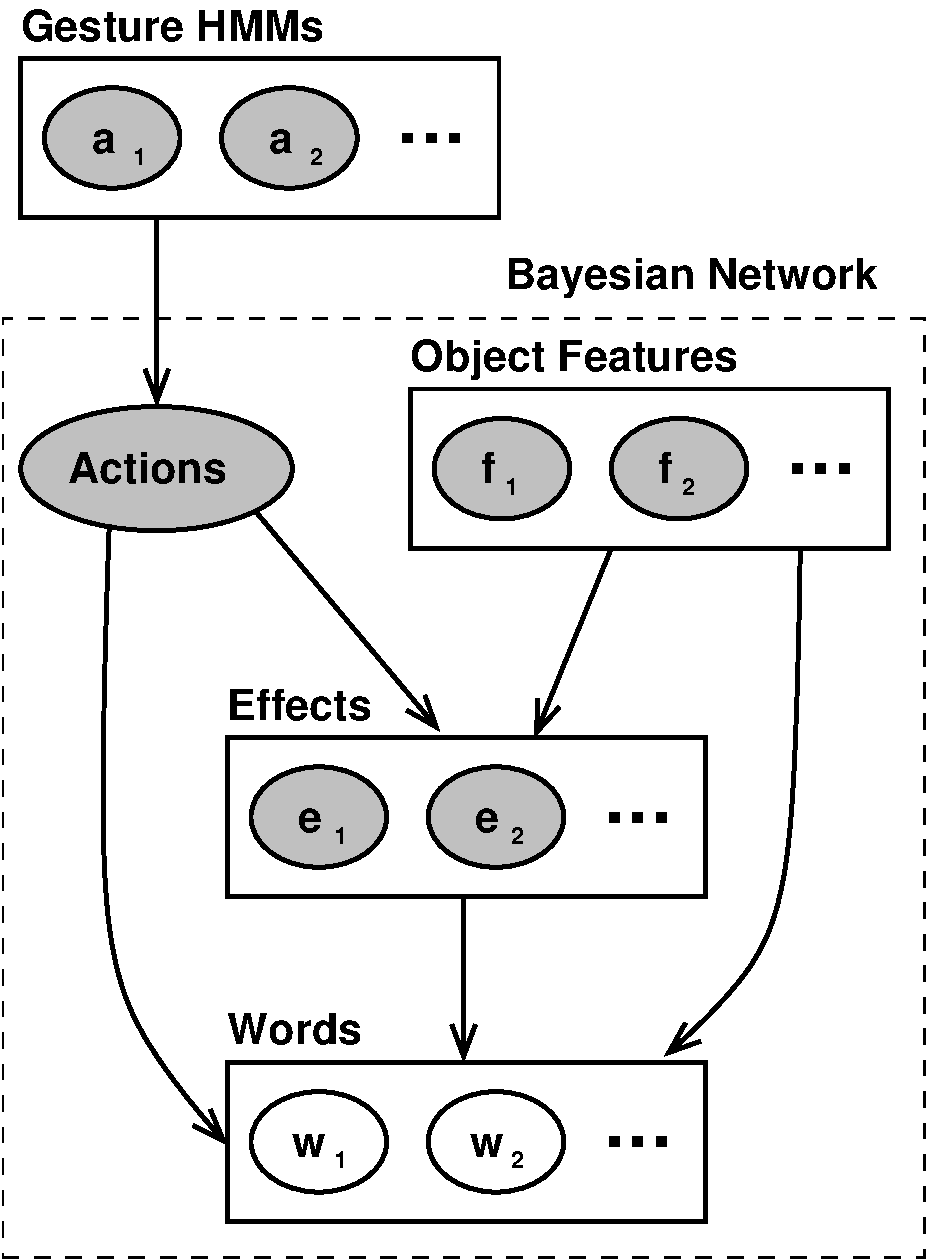
\includegraphics[width=0.8\columnwidth]{fullNetAbstract}
  \caption{Abstract representation of the probabilistic dependencies in the model. Shaded nodes are observable or measurable in the present study, and edges indicate Bayesian dependency.}
  \label{fig:model}
\end{figure*}

\section{Related Work}

BELOW IS THE GLU TEXT

A large and growing body of research is directed towards having robots learn new cognitive skills, or improving their capabilities, by interacting autonomously with their surrounding environment. In particular, robots operating in an unstructured scenario may understand available opportunities conditioned on their body, perception and sensorimotor experiences: the intersection of these elements gives rise to object affordances~(action possibilities), as they are called in psychology~\cite{gibson:2014}. The usefulness of affordances in cognitive robotics is in the fact that they capture essential properties of environment objects in terms of the actions that a robot is able to perform with them~\cite{montesano:2008,jamone:2016:tcds}.
Some authors have suggested an alternative computational model called \acp{OAC}~\cite{kruger:2011:ras}, which links low-level sensorimotor knowledge with high-level symbolic reasoning hierarchically in autonomous robots.

In addition, several works have demonstrated how combining robot affordance learning with language grounding can provide cognitive robots with new and useful skills, such as learning the association of spoken words with sensorimotor experience~\cite{salvi:2012:smcb,morse:2016:cogsci} or sensorimotor representations~\cite{stramandinoli:2016:icdl}, learning tool use capabilities~\cite{goncalves:2014:icarsc,goncalves:2014:icdl}, and carrying out complex manipulation tasks expressed in natural language instructions which require planning and reasoning~\cite{antunes:2016:icra}.

In~\cite{salvi:2012:smcb}, a joint model is proposed to learn robot affordances~(i.e., relationships between actions, objects and resulting effects) together with word meanings. The data contains robot manipulation experiments, each of them associated with a number of alternative verbal descriptions uttered by two speakers for a total of 1270~recordings. That framework assumes that the robot action is known a~priori during the training phase~(e.g., the information ``grasping'' during a grasping experiment is given), and the resulting model can be used at testing to make inferences about the environment, including estimating the most likely action, based on evidence from other pieces of information.

Several neuroscience and psychology studies build upon the theory of mirror neurons which we brought up in the Introduction. These studies indicate that perceptual input can be linked with the human action system for predicting future outcomes of actions, i.e., the effect of actions, particularly when the person possesses concrete personal experience of the actions being observed in others~\cite{aglioti:2008:basketball,knoblich:2001:psychsci}. This has also been exploited under the deep learning paradigm~\cite{kim:2017:nn}, by using a \ac{MTRNN} to have an artificial simulated agent infer human intention from joint information about object affordances and human actions. One difference between this line of research and ours is that we use real, noisy data acquired from robots and sensors to test our models, rather than virtual simulations.
